\chapter{Experimental Setup}
\label{ch:setup}

The following chapter describes the experimental setup for the discussion of results in chapter \ref{ch:discussion}. The first section of the chapter deals with data preprocessing. Section \ref{sec:05_Data} lists all datasets used for evaluations of the models and finally section \ref{sec:05_TrainingAndEvaluation} provides detail about the training and evaluation process used to generate the results.

\section{Data Preprocessing}
The following section describes the general data preprocessing steps which were taken for all datasets described in section \ref{sec:Data}. Some of the preprocessing steps are specific to certain datasets and will be described there. All data preprocessing steps can be enabled or disabled to evaluate the impact on the performance of these preprocessing steps. Some of those results will be discussed in section \ref{subsec:06_dataPreprocessing} in chapter \ref{ch:discussion}.

\subsection{Text Cleaning}
The main goal of the text cleaning step is 
\begin{enumerate}
	\item Reduce the number of words which are out of vocabulary
	\item Keep the vocabulary size as small as possible.
\end{enumerate}

without changing the semantics of the text.


The first step of the data preprocessing pipeline is the removal of all unknown characters which are not UTF-8 compatible. Those characters can occur because of encoding issues or words outside of the target language. 
\subsubsection*{Contraction Expansion}

Before we remove any special characters all contractions are expanded with the goal of reducing the vocabulary size and language normalization. Contractions are shortened versions of several words or syllables. In the English language, vowels are often replaced by an apostrophe.  Especially in social media and spoken language a lot of contractions are used. '\textit{I'll've}' and '\textit{I will have}' have the same meaning but if they are not expanded they produce a completely different embedding. '\textit{I'll've}' will produce a (300)-dimensional vector (for glove and fasttext) whereas '\textit{I will have}' will be interpreted as 3 300-dimensional vectors.

% TODO: Cite and/or check fasttext and glove naming

The contraction expansion is followed by the replacement of \glspl{url} with the token '<URL>' and e-mail addresses with the token '<MAIL>'. E-Mails and URLs are always out-of vocabulary and contain very little information that is worth encoding. 


In addition any special characters are completely removed. Dashes ('-') are kept because there are compound-words which rely on dashes (e.g. non-organic).

\subsubsection*{Spell Checking}
\label{sec:05_SpellChecking}
When writing comments in social media people tend to make spelling mistakes. Unfortunately, each spelling mistake is an out-of vocabulary word which we want to reduce as much as possible.

Therefore, a spell checker is used to prevent these mistakes. The first spell checker\footnote{PySpellchecker: \hyperlink{https://pyspellchecker.readthedocs.io/en/latest/}{https://pyspellchecker.readthedocs.io/en/latest/}} which was evaluated relies on the Levenshtein Distance \cite{Levenshtein1966} and a dictionary to determine if a word is spelled incorrectly and to make suggestions which word was meant originally. Although, word replacement suggestions are good, the spell checking is slow especially with large dictionaries.

The second spell checker is called Hunspell developed by László Németh\footnote{Hunspell: \hyperlink{http://hunspell.github.io/}{http://hunspell.github.io/}}. Hunspell is used in a variety of open- and closed sourced projects such as OpenOffice, Google Chrome or macOS. Hunspell also utilizes the Levenshtein Distance in addition to several other measurements. Both spell checkers suffer from false positives {(word is incorrectly flagged as negative)} as well as incorrect suggestions. Below are examples of Hunspells suggestions for words it did not recognize:

\begin{itemize}
	\item taste/flavor -> flavorless
	\item GMOs -> G Mos
	\item Coca~Cola -> Chocolate
	\item didn -> did
\end{itemize}

All of the above replacements are very bad because they change the meaning of the entire sentence.

Nevertheless, in terms of vocabulary size reduction they are clearly outperforming other techniques as table \ref{tab:05_amazonVocabSize} demonstrates. Running Hunspell on the Amazon dataset reduces the original vocabulary size of 1.6 Million by over 80\% to about 311,000 unique words. In addition, as column \textit{SP + TR-1} shows there are no tokens which only appear once. The reason for this is, that Hunspell always suggests something. Even words like \textit{\^{}\_\^{}b4} are replaced by new words even if it would make more sense to delete those words altogether.


\subsubsection*{Stemming and Lemmatization}

% TODO: cite and explain Stemming and Lemmatization
Stemming were also briefly explored, however, they did not provide a significant performance improvement.

\subsection{Comment Clipping}

% TODO: Show how many comments are very long in dataset

The transformer works with different input sequence lengths within one batch. Therefore, it is possible to group similar sequence lengths together and have arbitrary sequence lengths. Unfortunately, in each dataset there is a small percentage of sequences which are longer than other sequences. Due to the limited computational resources a batch of those long sequences  does not fit into \gls{gpu} memory. Therefore, all sentences are either padded or clipped to a fixed length. This is also a requirement for the CNN-based transformer aspect head since CNN-layers need a fixed number of input channels.

\subsection{Sentence Combination}

Some datasets feature sentence annotations instead of comment annotations. In this case important information for the aspect and sentiment classification could be encoded in previous sentences. Refer to figure XX for an example.

Therefore, $n$ previous sentences are prepended to the current sentence where $n$ is a hyper parameter which can be optimized. Similar to the clipping of comment wise annotations described in the previous section, these sentence combinations are also clipped and padded. 

The process starts by repeatedly adding sentences to a stack. All $n-1$ sentences which are too long are cut at the front. The $n$-th sentence is cut in the back instead. This is done so that in the case of $n=2$ 

% TODO: Show where sentiment is: analyise per word predictions and see if it makes sense to cut at the front or the back 

See section \ref{subsec:06_CommentClipping} for the evaluation of this preprocessing step.

\section{Data}
\label{sec:05_Data}


\subsection{Conll-2003 - Named Entity Recognition}
\subsection{GermEval-2017 - Deutsche Bahn Tweets}
\subsubsection*{Bahn Name Harmonization}
\subsection{Organic-2019 - Organic Comments}
\subsection{Amazon Reviews Dataset}

The Amazon Reviews Dataset consists of over 130 million Amazon product reviews from 1995 until 2015. Therefore, this dataset is one of the richest data sources for sentiment analysis or other related \gls{nlp} tasks. The raw data is available directly through amazon.\footnote{\hyperlink{https://s3.amazonaws.com/amazon-reviews-pds/readme.html}{https://s3.amazonaws.com/amazon-reviews-pds/readme.html}} The reviews are grouped into 45 product categories such as "Grocery", "Luggage" or "Video Games". 

In 2013 McAuley and Leskovec compiled a subset of Amazon reviews \cite{McAuley2013}. This dataset contains 34,7 million reviews ranging from 1995 till 2013 grouped into 33 categories\footnote{Available through Stanford \hyperlink{https://snap.stanford.edu/data/web-Amazon.html}{https://snap.stanford.edu/data/web-Amazon.html}}. The authors also created a "Fine Food" Dataset from Amazon reviews \cite{McAuley2013a} \footnote{Available through Kaggle \hyperlink{https://www.kaggle.com/snap/amazon-fine-food-reviews}{https://www.kaggle.com/snap/amazon-fine-food-reviews}}. This dataset consists of 568454 Amazon reviews from 1995 till 2012. The domain of this specific dataset is related to the organic domain with 273 occurrences of the word 'organic'. Unfortunately, it does not contain predefined aspects so \gls{absa} is not possible without extensive pre-processing to generate aspects out of the reviews.

The datasets created in 2013 contains duplicates so McAuley et. al. generated an improved Amazon Reviews dataset in 2015 without duplicates \cite{McAuley2015}\cite{He2016}. This iteration of the dataset contains 142.8 million reviews from 1996 till 2014\footnote{Available here: \hyperlink{http://jmcauley.ucsd.edu/data/amazon/}{http://jmcauley.ucsd.edu/data/amazon/}}. Due to the size of this dataset the authors provide a smaller dataset which only contains reviews from users who wrote exactly 5 reviews. This 5-core subset features 18 million reviews. The distribution of the domain categories is visualized in figure \ref{fig:05_amazonDatasetDistributin}. As one can observe the dataset is substantially skewed towards the largest domain 'books' which makes up of 49\% of the data.

\begin{figure}[ht]
	\centering
	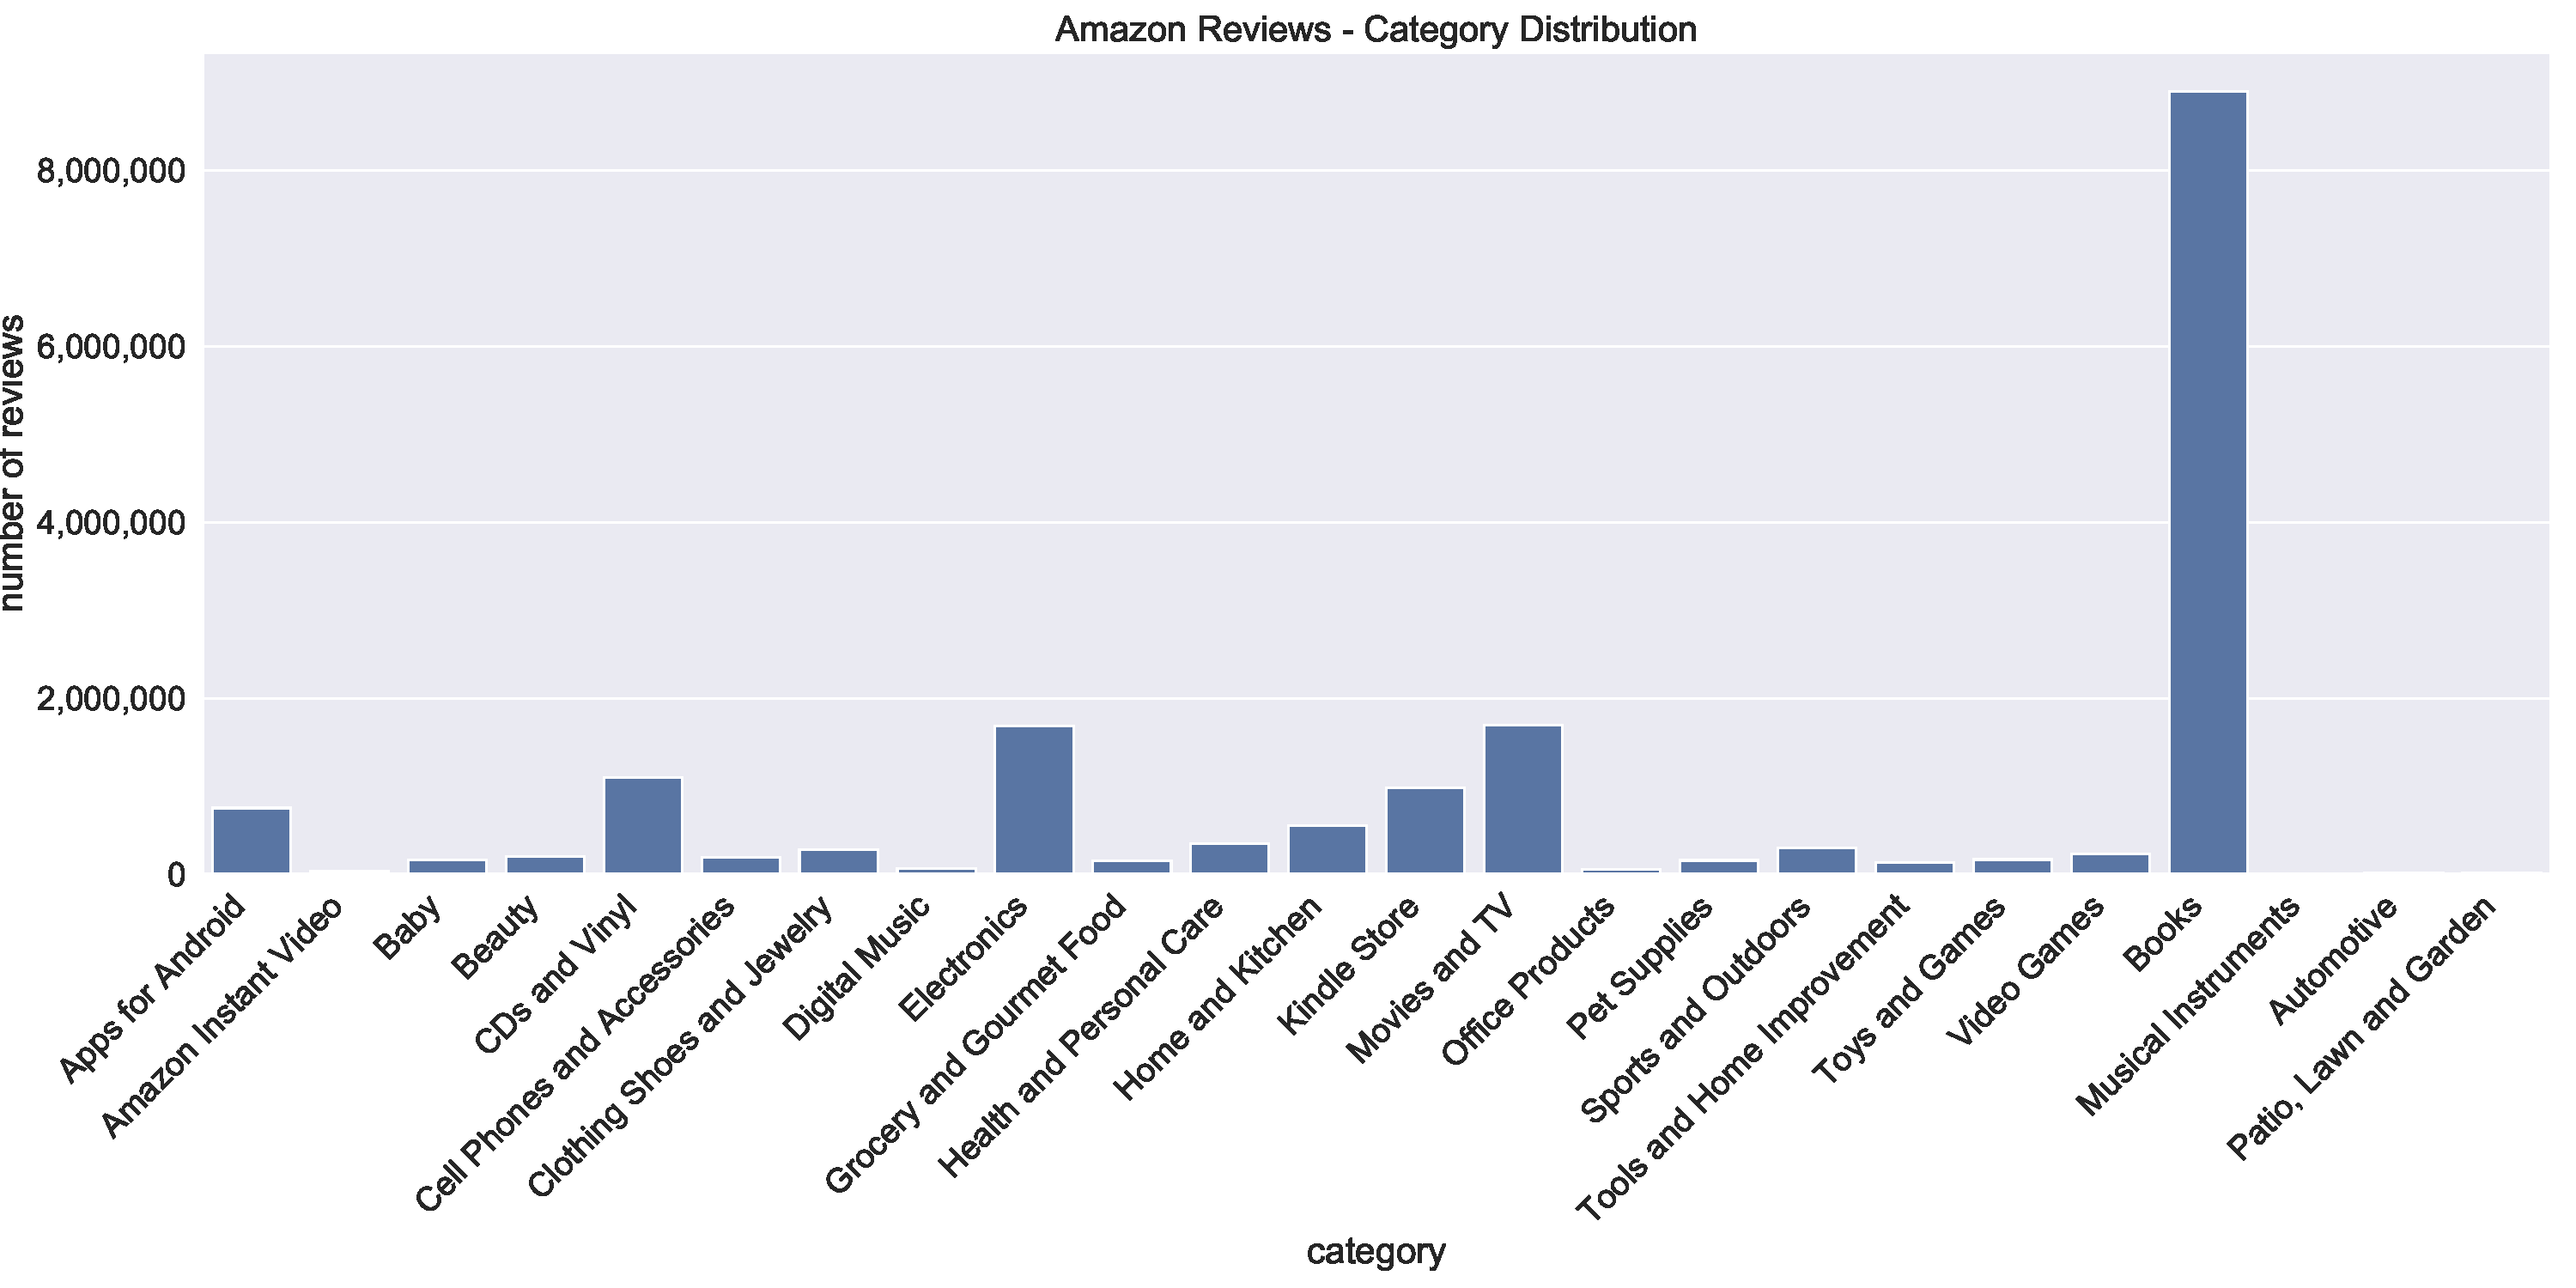
\includegraphics[width=\textwidth]{figures/05_setup/05_amazonReviewsCategories}
	\caption{Number of reviews per domain category in the amazon review dataset by McAuley et. al. \cite{McAuley2015}}
	\label{fig:05_amazonDatasetDistributin}
\end{figure}

To combat data imbalance and the sheer size of the dataset we propose a balanced subset of the 5-core dataset with 60000 reviews for each domain aside from \textit{Musical Instruments}, \textit{Amazon Instant Video}, \textit{Automotive} and \textit{Patio, Lawn and Garden}. These categories contain less than 50000 reviews so including them would skew the dataset again. In addition, we also transformed the star-rating to the common negative-neutral-positive rating schema. Similar to Blitzer et. al. we interpret $1-2$ stars as negative, 3 stars as neutral and $4-5$ stars as positive sentiment \cite{Blitzer2007}.

To create a balanced dataset not only on domains but also on sentiment we sampled 20000 reviews for each sentiment for each domain. Overall, there are more positive reviews than neutral or negative reviews. Thus, some domains contain less than 20000 reviews per sentiment category. To prevent data imbalance, reviews from the remaining other sentiment categories are sampled so that each domain contains 60000 reviews in sum. This distribution and additional statistics about the dataset are documented in table \ref{tab:05_amazonDatasetStats}.
\begin{table}	
	\begin{tabularx}{\textwidth}{lXrrrcrr}
		
		\toprule
		{} & helpful & \multicolumn{1}{c}{Pos.} & \multicolumn{1}{c}{Neu.} & \multicolumn{1}{c}{Neg.} &\multicolumn{1}{c}{stars} & \multicolumn{2}{c}{\# words} \\
		{} &         					mean &   	Count & Count & Count &  mean 	&  mean  &     std \\
		Domain Category             &        &            &       &       &       	&    	 &         \\
		\midrule
		Apps for Android            &   0.22 &   20000 &  	20000 & 20000 &    3.03 &     47 &   50 \\
		Baby                        &   0.29 & 	17012 &  	17255 &  	17012 &    3.33 &    105 &  106 \\
		Beauty                      &   0.32 &   20000 &  	20000 & 20000 &    3.10 &     90 &   94 \\
		Books                       &   0.43 &   20000 &  	20000 & 20000 &    3.08 &    176 &  201 \\
		CDs \& Vinyl                &   0.44 &   20000 &  	20000 & 20000 &    3.11 &    172 &  168 \\
		Cell Phones \& Accessories  &   0.19 &   20000 &  	20000 & 20000 &    3.06 &     93 &  138 \\
		Clothing Shoes \& Jewelry   &   0.26&   20000 &  	20000 & 20000 &    3.11 &     67 &   70 \\
		Digital Music               &   0.53 &  47410 &  	6789 &  5801 &    4.19 &    202 &  190 \\
		Electronics                 &   0.43 &   20000 &  	20000 & 20000 &    3.06 &    122 &  138 \\
		Grocery \& Gourmet Food     &   0.33 &  28790 & 17514 & 13696 &    3.53 &    99  &   97 \\
		Health \& Personal Care     &   0.35 &   20000 &  	20000 & 20000 &    3.09 &     95 &  126 \\
		Home \& Kitchen             &   0.44 &   20000 &  	20000 & 20000 &    3.08 &    104 &  110 \\
		Kindle Store                &   0.35 &   20000 &  	20000 & 20000 &    3.07 &    111 &  131 \\
		Movies \& TV                &   0.39 &   20000 &  	20000 & 20000 &    3.07 &    184 &  198 \\
		Office Products             &   0.29 &  45342 &  5060 & 2856 &    4.35 &    148 &  164 \\
		Pet Supplies                &   0.27 &  26412 & 15933 & 17655 &    3.35 &     91 &   96 \\
		Sports \& Outdoors          &   0.30 &  20751 & 20000 & 19249 &    3.14 &     94 &  111 \\
		Tools \& Home Impr.  		&   0.40 &  39126 & 10769 & 10105 &    3.90 &    111 &  134 \\
		Toys \& Games               &   0.32 &  11005 & 16357 & 11005 &    3.70 &    108 &  114 \\
		Video Games                 &   0.41 &   20000 &  	20000 & 20000 &    3.07 &    226 &  267 \\
		\midrule
		Total						&	0.35 & 	   506202 &	349677& 337379&    3.31 &	 122 &  151 \\
		\bottomrule
	\end{tabularx}
	\caption{Dataset statistics for the generated Amazon review subset for the domain categories. This table contains mean helpfulness rating; number of positive reviews; number of neutral reviews; number of negative reviews; mean star rating; mean number of words per review; standard deviation of the number of words per review }
		\label{tab:05_amazonDatasetStats}
\end{table}

\subsubsection*{Token Removal}
There are over 145 million words in the dataset. These words combine into a vocabulary size of 1.6 million unique tokens and consequently into a very large embedding layer. {(In comparison: the Organic2019 dataset has a vocabulary size of just 11,685.)} Two techniques were used to reduce the vocabulary size:

\begin{enumerate}
	\item Spell checking words
	\item Removing rare tokens
\end{enumerate}

The process for the first technique is described in section \ref{sec:05_SpellChecking}. Another way to reduce the vocabulary size is by removing tokens, that only occur once or twice. These tokens make up the majority of the vocabulary size but only a small percentage of the overall word count. Table \ref{tab:05_amazonVocabSize} shows the proportion of tokens which only occur 1, 2, or 3 times. As demonstrated in the table, infrequent tokens are very rare {(all the tokens with one occurrence make up only 0.33\% of the whole dataset)}. Yet, infrequent tokens make up over 74\% of the total vocabulary size. Removing all tokens with one occurrence, therefore reduces the vocabulary size by 74\% but only 0.33\% of information is lost.

Most of these rare tokens are either incorrectly written {(\textit{nthis})}, are part of structural elements such as headings {(\textit{review=======pros})} or are other unidentifiable characters and digits ({\textit{\^{}\_\^{}b4}}).

\begin{table}[]
	\centering
	\begin{tabular}{lrrrrrr}
			\toprule
							& Original  	& SP & SP + TR-1 & TR-1 & TR-2 & TR-3 \\
			\midrule
			Word Count      &148,129,490 	& -              & 0\%           & 0.329\%         & 0.389\%         & 0.414\%            \\
			Vocabulary Size & 1,594,742   	& 80.51\%        & 80.51\% 		 & 62.97\%         & 74.41\%         & 79.32\%      \\  
			\bottomrule 	
	\end{tabular}

	\caption{Different vocabulary size reduction techniques. This table shows the proportion of tokens that occur only 1, 2 or 3 times in relation to the total word count and the vocabulary size. \textit{SP} is the spell checked dataset; \textit{TR-}$n$ is the token removal technique were $n$ is the number times, tokens can occur in the dataset.}
	\label{tab:05_amazonVocabSize}
\end{table}

\section{Training and Evaluation}
\label{sec:05_TrainingAndEvaluation}

\subsection{Evaluation}

The models that are used in this thesis are stochastic models since model parameters are randomly initialized. In addition, samples within the training batches are randomly shuffled. Therefore running the model multiple times leads to different results.

This means that it is necessary to collect model results multiple times. Unfortunately, k-fold cross validation is not possible for three out of the four datasets since the creators of the datasets provide a predefined split and changing the split during k-fold cross validation would prevent comparability with other results.

Therefore, for each dataset-result we repeat the experiment 5-times and report the mean and standard deviation. Iyer and Rhinehart suggest to run an experiment up to a 1000 times to get an optimal result \cite{Iyer1999}. However, this is not possible for our models due to computational constraints.

All experiments on hyper parameters are performed once with a fixed seed of 42. This should make sure that all experiments on hyper parameters are reproducible. There are however some cudnn functions which are non-deterministic which means that even though a random seed is set the results could differ when running the same model with the same parameters multiple times.

\subsubsection*{GermEval 2017 - Evaluation}

Wojatzki et al. \cite{Wojatzki} provide an evaluation script for their dataset GermEval-2017. All results from the GermEval 2017 challenge were evaluated using this dataset. Therefore, all results reported in this thesis also use the evaluation script to calculate the f1 score. This is done to be able to compare the results on this datasets to other approaches on this data.

\begin{table}[hbt]
	\centering
	\label{tab:05_germevalEvaluationExample}
	\caption{Example for GermEval-2017 evaluation. None sentiment is not shown. Document 1 is predicted correctly. Document 2 has a correct prediction for aspect A but an incorrect prediction for the sentiment of aspect B {(in bold)}.}
	\begin{tabular}{@{}lcc}
		\toprule 
		& \textbf{Gold} & \textbf{Prediction} \\ 
		\hline 
		Document 1 & A : negative & A : negative \\ 
		\hline 
		\multirow{2}{*}{Document 2} & A : positive & A : positive \\ 
		& B : \textbf{positive} & B : \textbf{negative} \\ 
		\hline 
	\end{tabular}
\end{table}

Unfortunately, there are irregularities in the calculation of the micro f1 score. The evaluation script first creates every possible permutation of the combination of aspect and sentiment. If there are just two aspects {(Aspect A and Aspect B)} and four sentiments {(n/a, negative, neutral, positive)} this will generate 8 combinations {(A-n/a, A-negative, ..., B-positive)}. This is used as the first input {(\textit{aspect\_sentiment\_combinations})} of the GermEval-2017 evaluation algorithm shown in \ref{algo:05_germeval}.

In the next step, all gold-labels and predictions are paired together for each document based on the specific aspect-sentiment combination. The example in table \ref{tab:05_germevalEvaluationExample} will produce the following combinations where the left side represents the gold labels and the right side the predictions. This would be the second input parameter \textit{golds\_predictions} for algorithm \ref{algo:05_germeval}: 

\begin{enumerate}
	\item A:neg - A:neg (Document 1)
	\item A:pos - A:pos (Document 2)
	\item B:pos - B:n/a (Document 2)
	\item B:n/a - B:neg (Document 2)
\end{enumerate}

Using these inputs the algorithm will compute the following results:

\begin{itemize}
	\item True Positives: 2
	\item False Positives: 2
	\item False Negatives: 2
	\item True Negatives: 26
\end{itemize}

which results in an f1-score of $0.5$. In this example there is one misclassification where instead of predicting a pos. sentiment for aspect B the classifier predicted a neg. sentiment. When looking at the combination B:pos as the \textit{'true class'} the model predicts a negative {(NOT pos. sentiment)} when in reality this is a positive {(pos. sentiment)} which is the definition of a \textit{'False Negative'}. When looking at the combination B:neg as the \textit{'true class'} the model predicts a positive {(neg. sentiment)} when in reality this is a negative {(NOT neg. sentiment)} which is the definition of a \textit{' False Positive'}.

One could therefore argue that instead of producing two False Positives and two False Negatives the correct evaluation should be one False Positive and one False Negative.


\begin{algorithm}
	
	\SetKwInOut{Input}{Input}
	\SetKwInOut{Output}{Output}
	
	\Input{$aspect\_sentiment\_combinations$: List of all possible combinations between aspects and sentiments including n/a, $golds\_predictions$ List of all comment wise pairs between gold labels and prediction labels}
	\Output{($tp$, $fp$, $tn$ $fn$)}
	
	$tp$ = 0
	$fp$ = 0
	$tn$ = 0	
	$fn$ = 0
	
	\ForEach{($aspect$, $sentiment$) in $aspect\_sentiment\_combinations$}{
		\ForEach{($gold$), ($pred$) in  $golds\_predictions$}{
			
			\uIf{$gold$ matches current $aspect$ and $sentiment$}{
				\uIf{$gold$ matches $prediction$}{
					$tp$++
				} \Else {
					$fn$++
				}
			} \Else{
				\uIf{$prediction$ matches current $aspect$ and $sentiment$}{
					$fp$++
				} \Else{
					$tn$++
				}
			}
		}
		
	}
	
	\Return{(tp, fp, tn, fn)}
	
	\caption{GermEval-2017 Evaluation script.}
	\label{algo:05_germeval}
\end{algorithm}



\subsection{Hardware}

% TODO: Add hardware details
Training and evaluation of the models was done on four different machines. One of the servers belongs to the faculty of applied informatics, one is a local desktop machine and the last two are cloud instances. One is an Azure virtual compute instance with 8 \gls{cpu} cores and 28 \gls{gb} of \gls{ram} and the other is a Google Cloud \gls{gpu} compute instance instance with an Intel Xeon E5-2670 processor, 15 \gls{gb} of \gls{ram} and a NVIDIA Grid K520 \gls{gpu}. See table \ref{tab:05_usedHardware} for more details.
\begin{table}[hbt]
	\centering
	\caption{Hardware used for model training}
	\label{tab:05_usedHardware}
	\begin{tabular}{@{}ccccc@{}}
		\toprule
		\multicolumn{1}{c}{\textbf{}}    & \multicolumn{1}{c}{\textbf{OS}} & \multicolumn{1}{c}{\textbf{CPU}}                    & \multicolumn{1}{c}{\textbf{RAM}} & \multicolumn{1}{c}{\textbf{GPU}}     \\ \midrule
		Schlichter 2 & Ubuntu 12.04              & Intel Core i7-3930K @ 3.20GHz   & 63 GB        & NVIDIA Titan X \\ \midrule
		Schlichter 4 & Ubuntu 14.04              & Intel Xeon E5-2620 @ 2.00GHz    & 28 GB        & -                \\ \midrule
		Azure        & Ubuntu 15.10              & Intel Xeon E5-2673 v3 @ 2.40GHz & 28 GB        & -                \\ \midrule
		Amazon AWS   & Ubuntu 14.04              & Intel Xeon E5-2670              & 15 GB        & NVIDIA K520 \\ \bottomrule
	\end{tabular}
\end{table}


\subsection{Docker}
% TODO: Cite docker

% TODO: Explain Docker
Docker is a virtualization framework ...

% Add link to Docker Hub and image as footnote

Since training was performed on four different environments a Docker image was created which automates the installation of all required frameworks, environments, drivers and versions. An automated build pipeline builds a new image as soon as a new code version is pushed to the repository. Users can install or update an image directly from Docker Hub without rebuilding it every time locally.

The main concern of using docker for resource intensive task is the loss of performance due to the virtualization overhead. To evaluate this epoch training time was measured with and without docker. As one can observe in figure XX 

% TODO: measure epoch time with and without docker and report differences.


